\chapter{Conclusions} \label{chap:concl}

\section*{}

\section{Future Work}

In the time I'll be dedicated to accomplish what I have proposed to do, developing
a visual programming environment and gathering knowledge of what works best in
a visual representation and what doesn't, I'll be following the work plan presented
in Figure \ref{fig:workplan}.

During these nearly 5 months, the plan is to start weighting the pros and cons
of using certain PPLs and picking one of them to be used. The next step would be
picking an apropriate frontend, deciding between Blockly, a custom HTML+Javascript
solution, or other alternative. Then, I'll start by gathering the fundamental
language constructs that must be included, defining how they could be represented
in the visual language and developing the frontend and code generation for those constructs.
From this point onwards until the end, I've planned to make iterations: of choosing
new language features to integrate, adapt the frontend and code generation for them,
converting textual examples to the visual representation and studying the differences
between the two representations. Finnally, there
will be some time to make a tutorial on how to use the VPE.

\begin{figure}[t]
  \begin{center}
    \leavevmode
    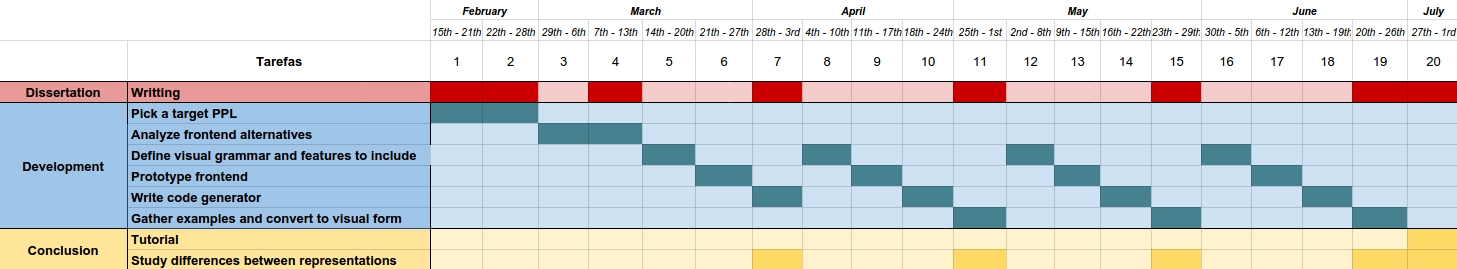
\includegraphics[width=0.86\textwidth]{workplan}
    \caption{Work plan for the work of this dissertation}
    \label{fig:workplan}
  \end{center}
\end{figure}
